\section{XSeparation Compiler}
\label{sec:compilation}
%XSeparation generates object-oriented code containing additional constructs for bidirectional traceability. Hence, a compilation process is needed to transform the XSeparation-generated code into machine code.
This section presents the architecture of the XSeparation compiler. %to transform the XSeparation-generated code into machine code.
\begin{figure}
	\centering
	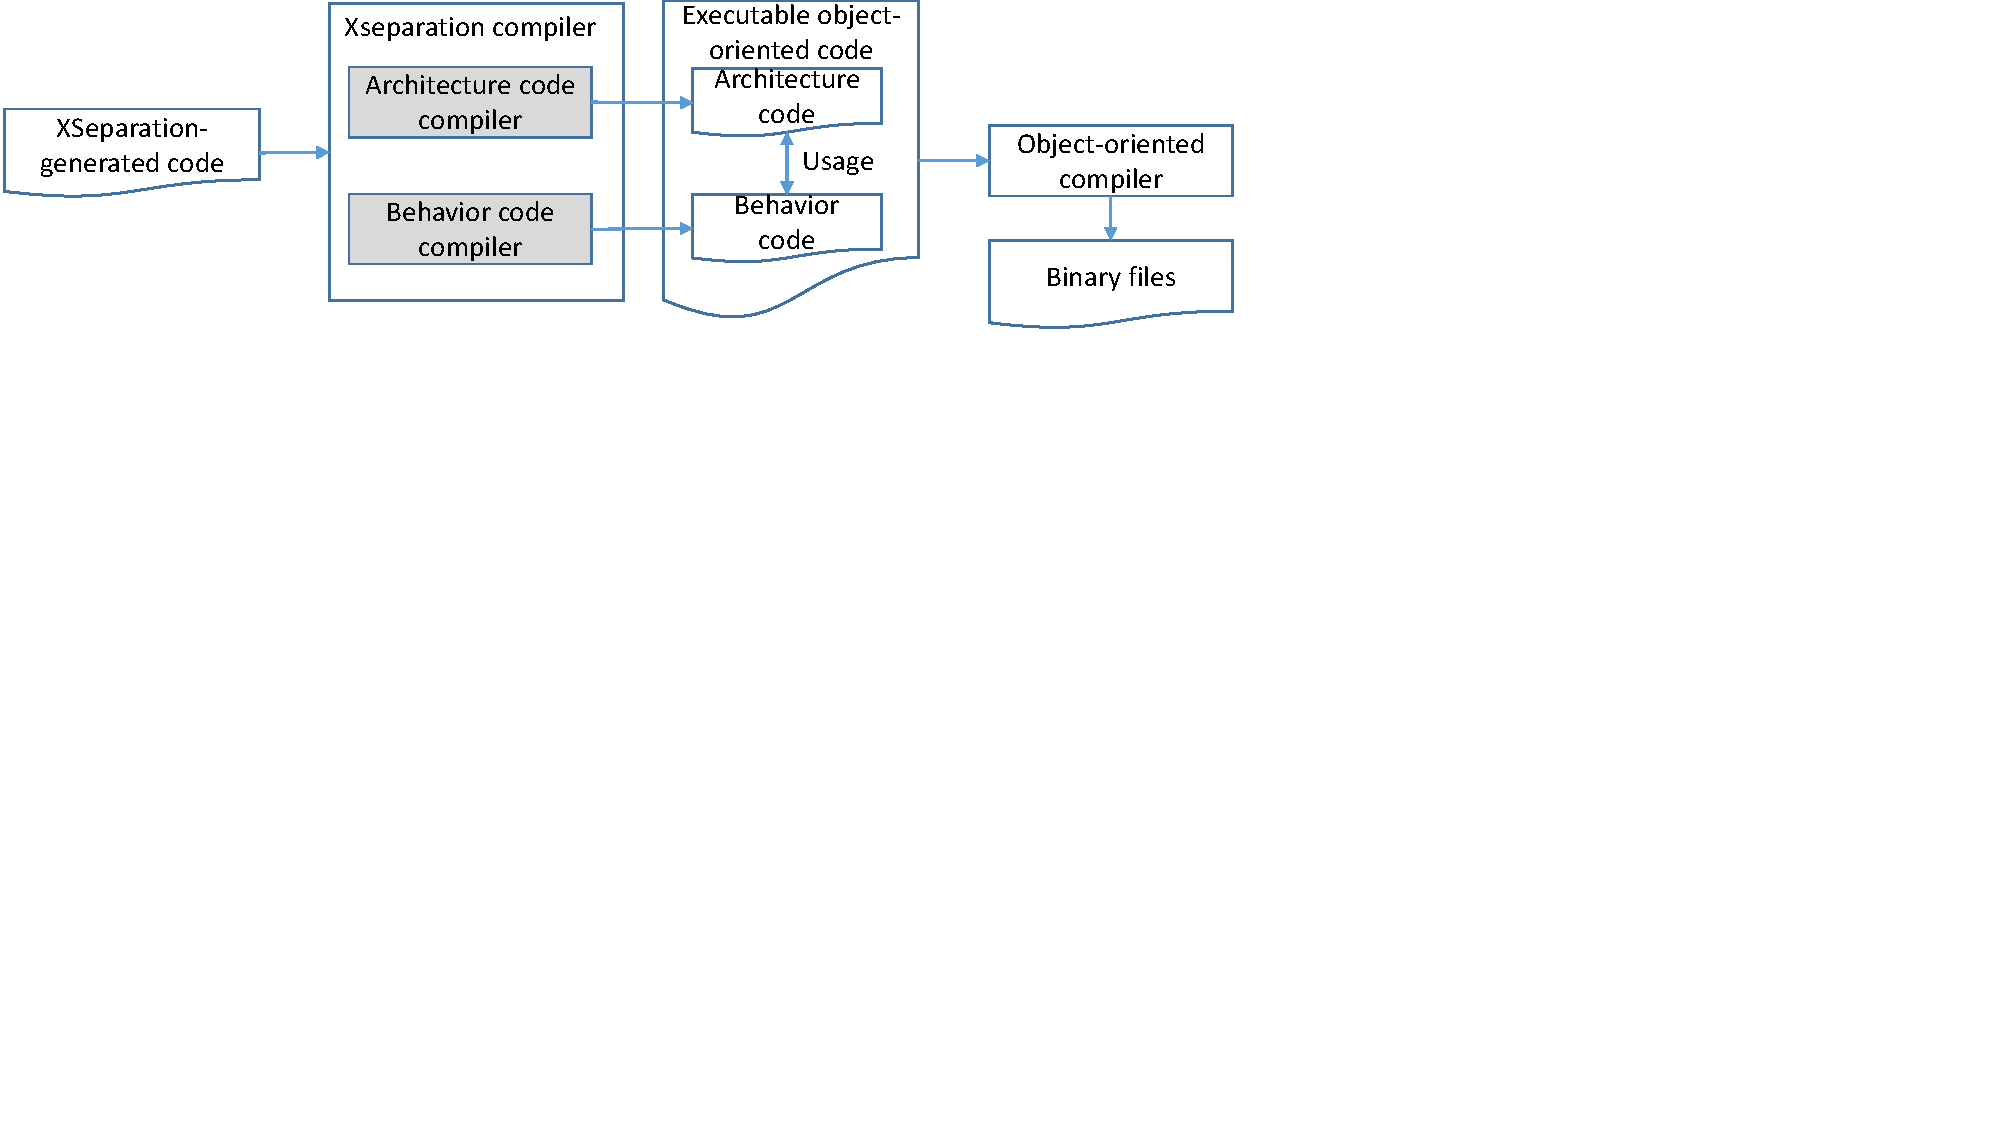
\includegraphics[clip, trim=0cm 13.3cm 12.8cm 0cm, width=\columnwidth]{figures/compilerarchitecture.pdf}
	\caption{XSeparation compiler's architecture} 
	\label{fig:compilerarchitecture}
\end{figure}
Fig. \ref{fig:compilerarchitecture} shows the compilation process, which takes as input the XSeparation-generated code, and produces the binary files by three two steps: \textcircled{1} generation of executable object-oriented code by the XSeparation compiler from XSeparation-generated code; \textcircled{2} production of binary files from the executable code by using object-oriented compilers such as GCC for C++ and Javac for Java.

The XSeparation compiler consists of two grayed sub-modules: \tb{Structure code compiler}, which takes as input the \tb{Component structure-prescribed code}, \tb{User-filled skeleton code}, and \tb{Component structure-provided implementation code} parts to produce \tb{Structure code}, while \tb{Behavior code compiler} takes as input the other parts to generate \tb{Behavior code}. 



\vskip 0.1cm
\noindent
\tb{Structure code compiler:}
A verification is firstly executed to check the well-formedness of components and ports.
We basically verify three port rules: (1) every port with a required interface or provided data must be bound to another port; (2) if two ports are connected by a assemble connector, the provided interface/data of one port must identical to or an extension of the required interface/data of the other port; and (3) if the connector is delegate, the provided interface/data of one port must identical to or an extension of the provided interface/port of the other port; 

Once the rules are verified, executable code can be generated. 
Listing \ref{lst:archcodecompiler} shows a \tb{Structure code} segment generated from the \ttt{System} example using ports with interfaces.
Each port is generated to a pointer attribute (lines 12 and 15) while each part to an object attribute (lines 3,4,5).
A configuration is transformed into a method named \ttt{configuration}.
When a method is called through a port as in Listing \ref{lst:producerinteraction}, for example \ttt{push} through the \ttt{pPush} port, the corresponding method implemented in FIFO is invoked. 

\begin{minipage}{\columnwidth}
	\lstinputlisting[language=C++, caption={Executable code generated by XSeparation compiler for the structure of \ttt{System}}, label=lst:archcodecompiler,frame=f]{code/archcodecompiler.cpp}
\end{minipage} 

\vskip 0.1cm
\noindent
\tb{Behavior code compiler:}
It generates executable code from the \tb{Behavior-prescribed code} and \tb{State machine action code} similarly to code generation approaches from UML State Machines in MDE tools such as Rhapsody and Sinelabore \cite{sinelabore}.
However, only a subset of UML State Machine concepts is supported by these tools, e.g. Rhapsody does not support junctions, and truly concurrent execution of orthogonal regions
\cite{ibmdiff} (see \cite{specification_uml_2007} for more detail) and the support for pseudo states such as history, choice and junction is poor \cite{EA, sinelabore}. 
%The concurrency of the orthogonal regions is often implemented sequentially \cite{Badreddin2014}. 
%In addition, there are other issues such as event processing speed, executable file size, and UML semantic-conformance defined by a recent work on the Precise Semantics of State Machine (PSSM) \cite{OMG2015}.
XSeparation compiler supports full features of state machines.
XSeparation compiler has following unique features:
\begin{itemize}[\footnotesize]
	\item \tb{Completeness:} XSeparation compiler supports all state machine vertexes and transitions including all pseudo states and transition kinds. 
	Hence, XSeparation compiler improves flexibility of using UML State Machines to express architecture behavior.
	For the moment, the only issue with the compiler is that it cannot deal with transitions from an entry point to an exit point.
	
	\item \tb{Event support:} XSeparation compiler utilizes four UML event types and deferred events, which are able to express synchronous and asynchronous behaviors and exchange data between components.
	
	\item \tb{UML-conformance:} A recent specification formalizing the precise semantics of UML State Machine is under standardization of OMG.
	It defines a test suite with 66 test cases for certifying the conformance of runtime execution of code generated from UML State Machines.
	We have experimented XSeparation compiler with the test suite.
	The traced execution results of 62/66 test cases comply with the standard and are a good hint that the execution is semantically correct.
	Due to space limitation, the details of patterns and evaluation for state machine code generation semantics are not presented in this paper.
	
	\item \tb{State machine configuration:} XSeparation allows to configure the event queue size and periodic time for evaluation of change events.
\end{itemize}


In the next section, XSeparation will be implemented as an extension of the Papyrus modeling tool and evaluated by developing a case study of software application for LEGO.